\documentclass{standalone}
\usepackage{tikz}

\begin{document}
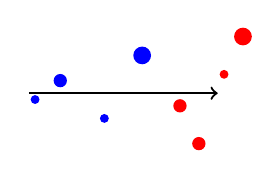
\begin{tikzpicture}[scale=0.8]

% Define colors
\definecolor{blueDot}{RGB}{0, 0, 255}
\definecolor{redDot}{RGB}{255, 0, 0}

% Draw the white arrow
\draw[thick, ->] (0,0) -- (3,0);

% Scatter blue and red dots around the arrow
\fill[blueDot] (0.1, -0.1) circle (2pt);
\fill[blueDot] (0.5, 0.2) circle (3pt);
\fill[blueDot] (1.2, -0.4) circle (2pt);
\fill[blueDot] (1.8, 0.6) circle (4pt);
\fill[redDot] (2.4, -0.2) circle (3pt);
\fill[redDot] (3.1, 0.3) circle (2pt);
\fill[redDot] (2.7, -0.8) circle (3pt);
\fill[redDot] (3.4, 0.9) circle (4pt);

\end{tikzpicture}
\end{document}